\section{Stack di monadi}
\label{sec:stack-di-monadi}

Come mostrato negli esempi riportati nella sezione precedente è possibile comporre gli effetti di più monadi tramite l'uso dei \term{monad transformer}. Ciascun \term{transformer} viene utilizzato per aggiungere la possibilità di effettuare uno specifico side effect a una monade di base: \lstinline{StateT} permette di aggiungere il side effect della modifica di uno stato, \lstinline{OptionT} permette di modellare il fallimento esplicito di una computazione.
Semplicemente osservando il \term{transformer} impiegato su una monade di base è possibile comprendere quali siano gli effetti aggiunti:
\begin{lstlisting}[language=scala3]
def program1: StateT[String, IO, Int] = ...
def program2: OptionT[IO, Int] = ...
\end{lstlisting}
\lstinline{program1} modella una computazione che può sia effettuare input e output che modificare uno stato mutabile di tipo stringa. Dal tipo di \lstinline{program2}, invece, è possibile dedurre che la computazione può fallire e che può effettuare input e output.

\subsection{Composizione di monadi}
Negli esempi mostrati fino ad ora è sempre stato applicato un singolo \term{transformer} a una monade di base. La monade risultante da questa composizione può avere due tipologie di side effect: quello della monade di base e quello aggiunto dal \term{transformer}.

Inoltre è possibile applicare più \term{transformer} ad una sola monade di base in modo da ottenere uno stack di monadi che possegga molteplici tipologie di side effect. Infatti, come emerge dalla definizione fornita in precedenza, un \term{transformer} è a sua volta una monade e nulla vieta di applicarvi un ulteriore \term{transformer}.
Si consideri per esempio la seguente monade definita utilizzando una serie di \term{transformer}:
\scalaFromFile{24}{24}{monads/transformers/Transformer.scala}
La monade \lstinline{Program} così definita permette di modellare una computazione che potrebbe fallire, modificare uno stato mutabile ed effettuare I/O. Dato che l'applicazione di \term{transformer} a una monade produce a sua volta una monade è possibile comporre un programma di tipo \lstinline{Program} sfruttando lo zucchero sintattico della \term{for comprehension}:
\scalaFromFile{25}{32}{monads/transformers/Transformer.scala}
La computazione descritta da questa porzione di codice legge una riga dallo \term{standard input}; se la stringa letta è \lstinline{"fail"} allora la computazione fallisce, altrimenti viene modificato lo stato mutabile impostandolo al valore della stringa.
È possibile utilizzare ciascuna delle azioni fornite dalle monadi di base -- in questo caso \lstinline{fail}, \lstinline{set} e \lstinline{getLine} -- previo un opportuno \term{lifting} per portarle nel livello corretto dello \term{stack} di monadi. In particolare:
\begin{itemize}
  \item L'operazione di lettura \lstinline{getLine} richiede un duplice \term{lifting}: poiché \lstinline{IO} è alla base dello \term{stack} di monadi il primo \lstinline{lift} servirà a portarlo nella monade \lstinline{StateT}; in questo modo è possibile ottenere un valore di tipo \lstinline{StateT[String, IO, String]}. Per poter portare tale valore dentro al transformer \lstinline{OptionT} è necessario applicare un'ultima volta l'operazione di \term{lifting}
  \item L'operazione di modifica dello stato richiede l'applicazione di \lstinline{lift} una sola volta dato che \lstinline{StateT} è nel secondo livello dello stack di monadi
  \item L'operazione di fallimento non richiede alcun \term{lifting}: \lstinline{fail} è già un valore di tipo \lstinline{OptionT} e pertanto può essere utilizzato direttamente
\end{itemize}

Per poter effettivamente eseguire una computazione descritta in questo modo è sufficiente utilizzare i metodi \lstinline{runStateT} e \lstinline{runOptionT}. Questi permettono di rimuovere i livelli dello \term{stack} di monadi fino ad arrivare ad una computazione che possa essere direttamente eseguita:
\scalaFromFile{34}{37}{monads/transformers/Transformer.scala}
Lo scopo della prima chiamata a \lstinline{runOptionT} è rimuovere il primo livello dello \term{stack} di monadi, ottenendo una computazione di tipo \lstinline{StateT[String, IO, Option[String]]}. La seconda chiamata a \lstinline{runStateT} -- fornendo il valore iniziale dello stato mutabile -- rimuove il secondo livello dello \term{stack} di monadi, ottenendo una computazione di tipo \lstinline{IO[(Option[Int], String)]}. Infine, la chiamata a \lstinline{unsafeRun} permette di eseguire la computazione ottenuta.

\subsection{Importanza dell'ordine nella composizione}
Come forse si sarà potuto intuire dall'esempio riportato in precedenza l'ordine con il quale vengono applicati i \term{transformer} svolge un ruolo fondamentale. In generale, modificare l'ordine delle monadi che compongono uno \term{stack} va a modificare la semantica del programma che si sta prendendo in considerazione. Per esempio, si considerino i seguenti \term{stack}:
\scalaFromFile{42}{43}{monads/transformers/Transformer.scala}
In \lstinline{Program2} è stato invertito l'ordine con cui sono stati applicati i due transformer. I due \term{stack} possono essere visualizzati come mostrato in \Cref{fig:transformers_stacks}:
\begin{itemize}
  \item \lstinline{Program1} rappresenta un programma che può effettuare I/O e potrebbe fallire. Nel caso in cui non fallisca la computazione può modificare uno stato mutabile; nel caso in cui invece la computazione fallisca allora sicuramente non potrà aver modificato lo stato globale
  \item \lstinline{Program2} rappresenta un programma che può effettuare I/O e modificare uno stato mutabile; il programma potrebbe non produrre alcun risultato fallendo ma avrebbe modificato in ogni caso lo stato globale
\end{itemize}

\begin{figure}[htp]
  \centering
  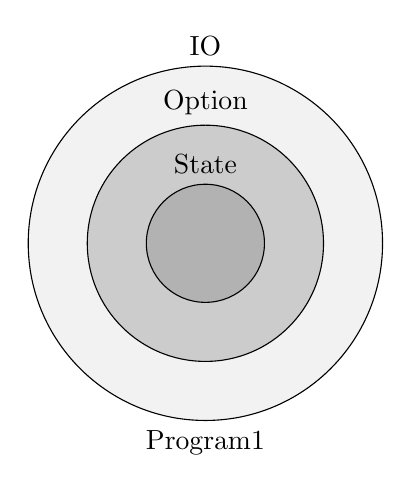
\begin{tikzpicture}
    \node[circle, fill=black!5, draw, minimum size=4.5 cm,label=above:{\lstinline{IO}}, label=below:{\lstinline{Program1}}] {};
    \node[circle, fill=black!20, draw, minimum size=3 cm,label=above:{\lstinline{Option}}] {};
    \node[circle, fill=black!30, draw, minimum size=1.5 cm,label=above:{\lstinline{State}}] {};
  \end{tikzpicture}
  \qquad
  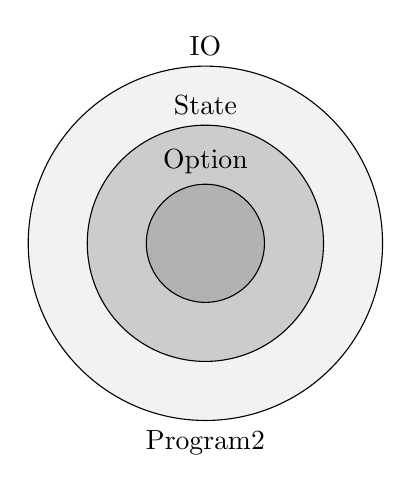
\begin{tikzpicture}
    \node[circle, fill=black!5, draw, minimum size=4.5 cm,label=above:{\lstinline{IO}}, label=below:{\lstinline{Program2}}] {};
    \node[circle, fill=black!20, draw, minimum size=3 cm,label=above:{\lstinline{State}}] {};
    \node[circle, fill=black!30, draw, minimum size=1.5 cm,label=above:{\lstinline{Option}}] {};
  \end{tikzpicture}
  \caption{Rappresentazione grafica degli stack di monadi corrispondenti ai tipi \lstinline{Program1} e \lstinline{Program2}}
  \label{fig:transformers_stacks}
\end{figure}


Quindi un valore di tipo \lstinline{Program1} può essere interpretato come una computazione che gestisce il proprio stato in maniera transazionale: si può accedere a uno stato mutabile ma in caso di fallimento della computazione non avviene alcune modifica. Al contrario, un valore di tipo \lstinline{Program2} potrebbe non produrre alcun risultato ma aver comunque modificato lo stato globale. Ciò è reso evidente dai tipi dei risultati ottenuti eseguendo le computazioni una volta eliminati i diversi livelli degli stack di monadi:
\scalaFromFile{45}{51}{monads/transformers/Transformer.scala}
L'esecuzione del primo programma ha come risultato un valore di tipo \lstinline{Option[(Int, String)]} -- dove il valore di tipo \lstinline{Int} è il risultato vero e proprio della computazione mentre quello di tipo \lstinline{String} rappresenta il nuovo stato. Quindi, nel caso in cui la computazione fallisca, non verrà prodotta una nuova versione dello stato mutabile che potrebbe essere stato modificato.
D'altro canto, l'esecuzione del secondo programma produce un valore di tipo \lstinline{(Option[Int], String)}: in questo caso, anche se la computazione dovesse fallire non producendo un risultato di valore \lstinline{Int}, sarebbe sempre presente una nuova versione dello stato mutabile.

\subsection{Miglioramento del parsing monadico}
Come mostrato in precedenza nella \Cref{sec:parsing-monadico} è possibile definire un \term{parser} con un'interfaccia monadica. Tuttavia si è potuto osservare come l'implementazione fornita presentasse una forte duplicazione di codice per reimplementare la logica delle monadi \lstinline{State} e \lstinline{Option}.
Grazie all'uso dei monad transformer è possibile ridefinire il tipo di un \term{parser} per eliminare completamente il codice duplicato:
\scalaFromFile{56}{56}{monads/transformers/Transformer.scala}

In questo modo non è più necessario dover derivare manualmente l'istanza di monade per \lstinline{Parser}: questa sarà ottenuta in automatico in virtù del fatto che un \lstinline{Parser} non è altro che uno \term{stack} di monadi.

Tuttavia, il fatto che \lstinline{Parser} sia implementato come uno \term{stack} di monadi rimane un dettaglio implementativo che è opportuno nascondere a chi fa uso di tale tipo. Per esempio si può definire un semplice \term{extension method} che permetta di effettuare il \term{parsing} di una stringa andando a rimuovere i livelli dello \term{stack} di monadi in maniera analoga a quanto mostrato in precedenza:
\scalaFromFile{57}{59}{monads/transformers/Transformer.scala}

Per esporre operazioni di base, come il fallimento del \term{parsing} o la lettura dello stato mutabile è possibile definire alcune funzioni che nascondano l'uso dei \term{transformer} che compongono lo \term{stack}:
\scalaFromFile{61}{64}{monads/transformers/Transformer.scala}

L'operazione di \term{parsing} di un singolo carattere dovrà quindi essere ridefinita in termini di queste operazioni di base:
\scalaFromFile{66}{74}{monads/transformers/Transformer.scala}

Le funzioni \lstinline{consumeTwo} e \lstinline{consumeN} mostrate in precedenza non necessitano di alcuna modifica in quanto sono state definite sulla base dell'interfaccia monadica di \lstinline{Parser} che, nella trasformazione dell'implementazione in uno \term{stack} di monadi, non è stata modificata.
